\begin{enumerate}[label=\thesubsection.\arabic*.,ref=\thesubsection.\theenumi]
\numberwithin{equation}{enumi}

\item Consider the parallel combination of two LTI systems shown in Fig. \ref{fig:ee18btech11029_block}, where
\begin{align}
h_1(t) &= 2\delta(t+2)-3\delta(t+1)
\\h_2(t) &= \delta(t-2)
\end {align}
%
 Find the transition matrix and the gain for this system.
\renewcommand{\thefigure}{\theenumi.\arabic{figure}}

%This is for generating the block diagram using Tikz
\usetikzlibrary{arrows,positioning,shapes.geometric}
\tikzstyle{sum} = [draw, circle, node distance=0.32cm]
\tikzstyle{output} = [coordinate]  
\tikzstyle{input} = [coordinate]
    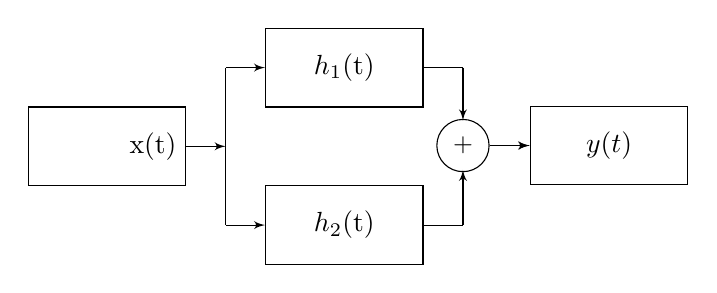
\begin{tikzpicture}[>=latex']
        \tikzset{block/.style= {draw, rectangle, align=center,minimum width=2cm,minimum height=1cm},
        }
        \node (start) {x(t)}; 
        \node [coordinate, name=input] {x(t)}; 
        \node [coordinate, right = 0.5cm of start] (ADL){};
        \node [block, left = 0.5cm of ADL] (A4){};
        \node [coordinate, above = 1cm of ADL] (AUL){};
        \node [coordinate, right = 0.5cm of start] (BUL){};
        \node [coordinate, below = 1cm of BUL] (BDL){};
        \node [block, right = 0.5cm of AUL] (A1){$\text{h}_\text{1}$(t)};
        \node [block, right = 0.5cm of BDL] (B1){$\text{h}_\text{2}$(t)};
        \node [coordinate, right = 0.5cm of ADL] (A2){$\text{h}_\text{1}$(t)};
        \node [coordinate, right = 0.5cm of A1] (APL){};
        \node [coordinate, right = 0.5cm of B1] (SPL){};
        \node [coordinate, below = 0.67cm of APL] (APM){};
        \node [coordinate, above = 0.7cm of SPL] (SPM){};
        \node [sum, below of=APM] (APN) {\small +};
        \node [coordinate, right = 0.5cm of APN] (APO){$y(t)$};
        \node [block, right = 0.01cm of APO] (A3){$y(t)$};
        
     \usetikzlibrary{arrows}   
        \draw [-]   (ADL) -- (AUL);
        \draw [->]   (AUL) -- (A1);
        \draw [-]   (A1) -- (APL);
        \draw [->]   (APL) -- (APM);
        \draw [-]   (APM) -- (APN);
        \draw [->]   (APN) -- (APO);
        \draw [->]   (APO) -- (A3);
        \draw [->]   (start) -- (BUL);
        \draw [-]   (BUL) -- (BDL);
        \draw [->]   (BDL) -- (B1);
        \draw [-]   (B1) -- (SPL);
        \draw [->]   (SPL) -- (SPM);
         
 \end{tikzpicture}
%
\\
\solution The signal flow graph for Fig. \ref{} is available in Fig. \ref{}.

\usetikzlibrary{decorations.markings}
\newif\iflabrev
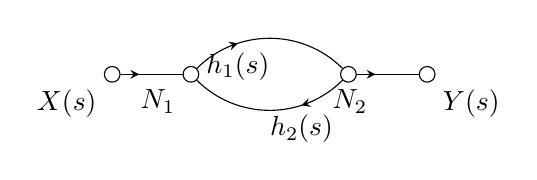
\begin{tikzpicture}
[
label revd/.is if=labrev,
%label revd/.default=true,
amark/.style={
            decoration={             
                        markings,   
                        mark=at position {0.3} with { 
                                    \arrow{stealth},
                                    \iflabrev \node[above] {#1};\else \node[below] {#1};\fi
                        }
            },
            postaction={decorate}
},
terminal/.style 2 args={draw,circle,inner sep=2pt,label={#1:#2}},
]

\node[terminal={below left}{$X(s)$}] (b) at (2cm,0) {};
\node[terminal={below left}{$N_1$}] (c) at (3cm,0) {};
\node[terminal={[xshift=-4mm]below right}{$N_2$}] (d) at (5cm,0) {};
\node[terminal={below right}{$Y(s)$}] (e) at (6cm,0) {};

\draw[amark= ] (b) to (c);
\draw[amark=$h_1(s)$] (c) to [bend left=45](d);
\draw[amark= ] (d) to (e);
\draw[amark=$h_2(s)$ ] (d) to[bend left=45] (c);


\end{tikzpicture}

\renewcommand{\thefigure}{\theenumi}

%
The transition matrix is then obtained as
\begin{align}
\vec{T} &= \myvec{0 & 0 \\
H_1(s) + H_2(s)& 0}
\\
\vec{T} &= \myvec{0 & 0 \\
2e^{2s} - 3e^{s} + e^{-2s}& 0}
\\
\implies \vec{I}-\vec{T} &= \myvec{1 & 0 \\
 -(2e^{2s} - 3e^{s} + e^{-2s}) & 1 }
\end{align}
%
Letting
\begin{align}
    \vec{U}=\brak{\vec{I}-\vec{T}}^{-1}
\end{align}

 \begin{align}
     H(s)=2{e^{2s}} - 3{e^{s}} + {e^{-2s}}
 \end{align}
%
\item Find the step response of the system and its energy.
\\
\solution 
 \begin{align}
     Y(s)&=X(s)H(s)
\\
     Y(s)&=\frac{2e^{2s}}{s} - \frac{3e^{s}}{s} + \frac{e^{-2s}}{s}
\\
\implies  y(t)&=2u(t+2)-3u(t+1)+u(t-2) \quad \text{and}
\\
y^2(t) &=
 \end{align}
%
which is sketched in Fig. \ref{fig:ee18btech11029_verify} by
\begin{lstlisting}
codes/ee18btech11029.py
\end{lstlisting}
%
 The desired energy is then obtained by computing the area as 7.
\begin{figure}
\centering
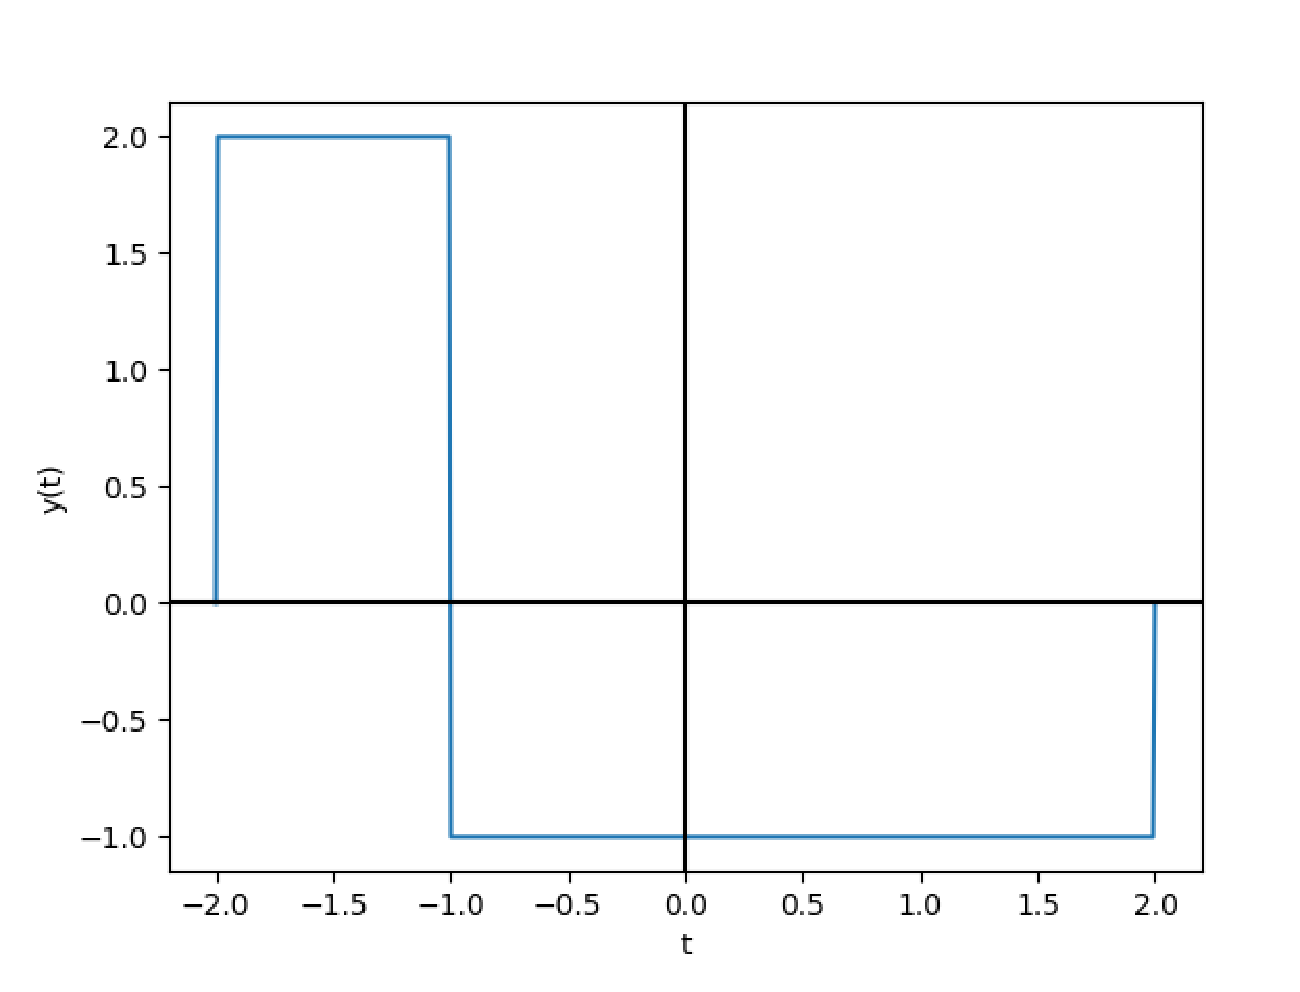
\includegraphics[width=\columnwidth]{./figs/ee18btech11029/verify.eps}
\caption{}
\label{fig:ee18btech11029_verify}
\end{figure}
\end{enumerate}

